% Some LaTeX commands I define for my own nomenclature.
% If you have to, it's better to change nomenclature once here than in a 
% million places throughout your thesis!
\newcommand{\package}[1]{\textbf{#1}} % package names in bold text
\newcommand{\cmmd}[1]{\textbackslash\texttt{#1}} % command name in tt font 


%======================================================================
\chapter{Observations}
%======================================================================

This would be a good place for some figures and tables.

Some notes on figures and photographs\ldots

\begin{itemize}
\item A well-prepared PDF should be 
  \begin{enumerate}
    \item Of reasonable size, {\it i.e.} photos cropped and compressed.
    \item Scalable, to allow enlargment of text and drawings. 
  \end{enumerate} 
\item Photos must be bit maps, and so are not scaleable by definition. TIFF and
BMP are uncompressed formats, while JPEG is compressed. Most photos can be
compressed without losing their illustrative value.
\item Drawings that you make should be scalable vector graphics, \emph{not} 
bit maps. Some scalable vector file formats are: EPS, SVG, PNG, WMF. These can
all be converted into PNG or PDF, that pdflatex recognizes. Your drawing 
package probably can export to one of these formats directly. Otherwise, a 
common procedure is to print-to-file through a Postscript printer driver to 
create a PS file, then convert that to EPS (encapsulated PS, which has a 
bounding box to describe its exact size rather than a whole page). 
Programs such as GSView (a Ghostscript GUI) can create both EPS and PDF from PS files.
Appendix~\ref{ch:Appendix-Matlab} shows how to generate properly sized Matlab plots and save them as PDF.
\item It's important to crop your photos and draw your figures to the size that
you want to appear in your thesis. Scaling photos with the 
includegraphics command will cause loss of resolution. And scaling down 
drawings may cause any text annotations to become too small.
\end{itemize}
 
For more information on \LaTeX\, see the uWaterloo Skills for the Academic Workplace 
course notes at \href{http://saw.uwaterloo.ca/latex}{saw.uwaterloo.ca/latex}. 
\footnote{
Note that while it is possible to include hyperlinks to external documents,
it is not wise to do so, since anything you can't control may change over time. 
It \emph{would} be appropriate and necessary to provide external links to 
additional resources for a multimedia ``enhanced'' thesis. 
But also note that if the \package{hyperref} package is not included, 
as for the print-optimized option in this thesis template, any \cmmd{href} 
commands in your logical document are no longer defined.
A work-around employed by this thesis template is to define a dummy \cmmd{href} 
command (which does nothing) in the preamble of the document, 
before the \package{hyperref} package is included. 
The dummy definition is then redifined by the
\package{hyperref} package when it is included.
}

The classic book by Leslie Lamport~\cite{lamport.book}, author of \LaTeX , is worth a look too, and the many available add-on packages are described by 
Goossens \textit{et~al.}~\cite{goossens.book}. Some on-line documentation is linked
to from \href{http://saw.uwaterloo.ca/latex}{saw.uwaterloo.ca/latex}. 



Here is an example of how to include figures in \LaTeX. 
Figure~\ref{fig.beam} shows a cantilever beam of circular cross-section
subjected to a point load and a uniformly distributed load, both of which are uncertain. Note that it is better not to include the extension of the figure's source file.

\begin{figure}[!htbp]
 \begin{center}
  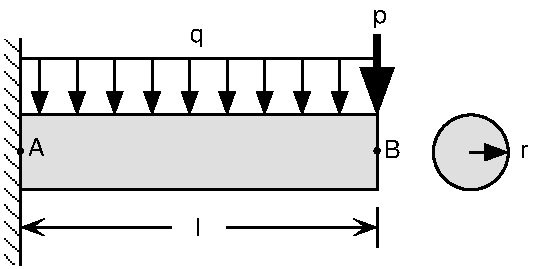
\includegraphics[clip=true]{figs/ipe/beam}
 \end{center}
\caption{Cantilever Beam}
\label{fig.beam}
\end{figure}



%----------------------------------------------------------------------
\section{Adding Nomenclature}
%----------------------------------------------------------------------

The following example is part of the ``nomentbl'' package. Refer to the package's documentation for more details.

\bigskip

\noindent
Let's start with equations to show how to use greek and mathematical symbols within Nomenclature.

Here is an equation
%
\begin{equation}\label{eq:heatflux}
  \dot{Q} = k \cdot A \cdot \Delta T
\end{equation}%
%
%% Greek and math symbols
% \nomenclature[gQ]{$\dot{Q}$}{heat flux}{W}{}%
% \nomenclature[gk]{$k$}{overall heat transfer coefficient}{$\frac{\mathrm{W}}{\mathrm{m}^2\mathrm{K}}$}{see eq.~(\ref{eq:ohtc})}%
% \nomenclature[gA]{$A$}{area}{m$^2$}{$L^2$}%
% \nomenclature[gL]{$L$}{length}{m}{SI base quantity}%
% \nomenclature[gT]{$T$}{temperature}{K}{SI base quantity}%
% \nomenclature[gT]{$\Delta T$}{temperature difference}{K}{SI base quantity}%

% Here is another one
% %
% \begin{equation}\label{eq:ohtc}
%   \frac{1}{k} = \left[\frac{1}{\alpha _{\mathrm{i}}\,r_{\mathrm{i}}} +
%     \sum^n_{j=1}\frac{1}{\lambda _j}\,
%     \ln \frac{r_{\mathrm{a},j}}{r_{\mathrm{i},j}} +
%     \frac{1}{\alpha _{\mathrm{a}}\,
%       r_{\mathrm{a}}}\right] \cdot r_{\mathrm{reference}}
% \end{equation}%
% %
% %% Greek and math symbols
% \nomenclature[ga]{$\alpha$}{convection heat transfer coefficient}{$\frac{\mathrm{W}}{\mathrm{m}^2\mathrm{K}}$}{}%
% \nomenclature[gl]{$\lambda$}{thermal conductivity}{$\frac{\mathrm{W}}{\mathrm{m K}}$}{}%
%
%% Subscripts
% \nomenclature[za]{a}{out}{}{}%
% \nomenclature[zi]{i}{in}{}{}%
% \nomenclature[zj]{$j$}{running parameter}{}{}% 
% \nomenclature[zn]{$n$}{number of walls}{}{}%


% \bigskip

% \noindent
% The following example is to show how to use abbreviations within the Nomenclature.\\
% EECS is a school at the UO.
% %% Abbreviations
% \nomenclature[a]{EECS}{Electrical Engineering and Computer Science}{}{}%
% \nomenclature[a]{UO}{University of Ottawa}{}{}%



\bigskip

\noindent
Don't forget to run:
\begin{verbatim}
makeindex -s nomentbl.ist -o uottawa-thesis.nls uottawa-thesis.nlo
\end{verbatim}



%%% Local Variables:
%%% mode: latex
%%% TeX-master: "../finalReportMainV1"
%%% End:
